\title{Matched Source Waveform Inversion for Transmitted Waves}
\author{Huiyi Chen, Susan E. Minkoff, and William W. Symes}

\lefthead{Symes}

\righthead{MSWI}

\maketitle
\parskip 12pt

\begin{abstract}
Matched Source Waveform Inversion applied to acoustic transmission data
produces an estimate of refractive index similar to the result of
travel time inversion, but without explicit identification of travel
times. This paper reviews the theoretical justification of this result
and its limitations, and with 2D numerical illustrations. 
\end{abstract}
\setlength{\parindent}{0cm}

\section{Introduction}
Matched Source Waveform Inversion (MSWI) is a variant of Full Waveform
Inversion (FWI) \cite[]{VirieuxOperto:09}, that sometimes overcomes
one of FWI's impediments, namely its tendency to stagnate at
suboptimal model estimates (``cycle-skip''), demonstrably far from global optima in
controlled settings and often uninformative of material structure in
field use. It is possible that such local descent algorithms are
trapped in regions around local minima, though such trapping, or even
the existence of local, non-global minima, are seldom established with
any rigor. MSWI
loosens the bond between predicted and observed data by interposing a
filter, adapted to map one to the other trace-by-trace, and penalizes
deviation of the filter from the Dirac delta. This soft penalty
effectively relaxes the FWI data-fitting problem and permits local
optimization methods to approximate data kinematics.

The aim of this paper is to review the theoretical basis of MSWI,
describe a practical computational framework for MSWI, and use it to
solve a synthetic acoustic inversion problem for which FWI fails. In
contrast, MSWI starting at the same initial estimate delivers an
improved velocity from which FWI succeeds in approaching the global
minimizer. The example is representative of a case (single arrival or
simple wavefront transmitted wave data) in which the MSWI objective
function is demonstrably close to mean square travel time error. Since
travel time inversion is generally not subject to cycle-skipping,
successful inversion is expected, and that is what we observe.

MSWI in the form described here was introduced by
\cite{HuangSymes2015SEG,HuangSymes:Geo17}. It is mathematically
equivalent to an {\em extended} formulation of the inverse problem, in
which acoustic point sources are allowed to depend on the receiving
sensors - a non-physical expansion of the simulation domain. A number
of other variants of FWI have been based on essentially the same
extension of acoustic modeling
\cite[]{Song:94c,Symes:94c,Plessix:00,LuoSava:11,LiAlkhalifah:21}. In
particular it is the basis of Adaptive Waveform Inversion (AWI) \cite[]{Warner:16,
  GuaschWarnerRavaut:GEO19,Warneretal:SEG21, Guaschetal:NPJDM20}. MSWI
is closely related to AWI, but not identical: AWI includes a
normalization of the adaptive filter, which makes the AWI objective
function an even closer approximation to travel time mean square error
than is MSWI, at least for transmitted wave data with a single
arriving wavefront \cite[]{Symes:24a}.

Transmission data with a single arrival is not just a case in which
MSWI and AWI are known to closely approximate travel time inversion:
it is the only case in which this link occurs. In particular, the link
is broken for transmission data exhibiting multiple arrivals: in the
presence of complex wavefronts, methods based on the source-receiver
extension are no less likely than FWI to cycle-skip
\cite[]{Symes:94c,HuangSymes:Geo17,Symes:24a}. However, the
source-receiver extension is not the only possible route to FWI
modification by artificially expanding the definition of energy
source. \cite{HuangNammourSymesDollizal:SEG19} overview modifications
of FWI based on various source extensions; some more recent advances
are described by
\cite{MetivierBrossier:SEG20,PladysBrossierLiMetivier:GEO21,LiAlkhalifah:21,Yongetal:GJI23,Opertoetal:GEO23}.
Numerical examples suggest that some of these extensions may avoid
cycle-skipping for transmitted wave data with complex wavefronts.

The next section describes versions of FWI and MSWI based on
acoustic wave propagation. The theoretical connection between MSWI and
travel time inversion is reviewed. The computations required to apply local
optimization to the objective functions of these inversion methods are
detailed, as is the variable projection reduction of MSWI and the use
of weighted norms in the domain of the simulation operator (wave
velocity or bulk modulus fields, in the setting developed here). The
third section presents an example, along with a detailed description
of the numerical methods for simulation and optimization methods used
in treating this example. The final section discusses some of the many
unresolved questions around MSWI and similar approaches to inverse
problems in wave propagation.

\section{Theory}
The version of MSWI discussed here uses acoustic wave propagation with
isotropic point sources and receivers.
The pressure and velocity fields $p({\bf x},t;{\bf x}_s)$, ${\bf v}({\bf x},t;{\bf x}_s)$ for the source location ${\bf x}_s$ depend on the bulk modulus $\kappa({\bf x})$, buoyancy $\beta({\bf x})$ (reciprocal of the density $\rho({\bf x})$), and wavelet $w(t;{\bf x}_s)$ through the acoustic system
\begin{eqnarray}
  \label{eqn:awe}
 \frac{\partial p}{\partial t} & = &- \kappa \nabla \cdot {\bf v} +
w(t;{\bf x}_s) \delta({\bf x}-{\bf x}_s); \nonumber \\
\frac{\partial {\bf v}}{\partial t} & = & - \beta \nabla p; \\ 
p, {\bf v} & = & 0 \mbox{ for }  t \ll 0.
\end{eqnarray}
The model vectors $m=(\kappa,\rho)$ make up the domain of the forward
map or {\em modeling operator} is $F[m]w = \{p({\bf x}_r,t;{\bf
  x}_s)\}$, for specified source and receiver positions ${\bf x}_s, {\bf x}_r$ and
recording interval $[0,t_d]$.

In the discussion that follows, the buoyancy $\beta$ will be regarded
as a fixed parameter. Thus $m$ is effectively the bulk modulus field $\kappa$.

In this context, FWI means: given source wavelet
$w(t;\bx_s)$ and data traces $d(\bx_r,\cdot;\bx_s)$, find a model $m$
so that $F[m]w \approx d$. The
simplest version of FWI concretizes this task by asking for a model
$m$ minimizing the mean square error
\begin{equation}
  \label{eqn:fwi}
  J_{\rm FWI}[m;d]= \frac{1}{2}\|F[m]w-d\|^2.
\end{equation}
Note that $w$ is assumed known and treated as a parameter in this
statement of the FWI task. In practice, it is not known (nor are the
sources and receviers necessarily isotropic), and should be estimated
along with the model $m$.

The approach to local optimization taken here (and in most work on FWI
and related topics) is based on the gradient of the objective defined
in equiation \ref{eqn:fwi}:
\begin{equation}
  \label{eqn:fwigrad}
  g = \nabla  J_{\rm FWI}[m;d] = D_m(F[m]w)^T(F[m]w-d).
\end{equation}
In this formula, $D_m(F[m]w)$ is the derivative of $F[m]w$ with
respect to $m$. 
This is the Euclidean (or $L^2$) gradient, that is, the vector $g$ for
which the Euclidean inner product
\begin{equation}
  \label{eqn:eucip}
  \langle g, \delta m\rangle = g^T\delta m
\end{equation}
with any other vector $\delta m$ gives the
rate of change in the direction of that vector of $J_{\rm FWI}$ at $m$.

For optimization within a set of slowly varying models (on the
wavelength scale),  it is appropriate to penalize oscillation of the
search vector. A convenient way to accompish this goal is the use of a
{\em weighted inner product} to define the gradient, rather than the
Euclidean inner product. A weight operator $W$ should be symmetric and
positive definite: then
\begin{equation}
  \label{eqn:wip}
  \langle g, \delta m\rangle_W = g^TW\delta m
\end{equation}
defines an alternative inner product. Comparing the definitions
\ref{eqn:fwigrad}, \ref{eqn:eucip}, and \ref{eqn:wip}, clearly the
vector $g_W$ for which $\langle g_W, \delta m \rangle_W$ gives the
rate of change of $J_{\rm FWI}$ at $m$ in the direction $\delta m$ is
\begin{equation}
  \label{eqn:fwiwgrad}
  g_W = W^{-1}\nabla  J_{\rm FWI}[m;d] =W^{-1} D_m(F[m]w)^T(F[m]w-d).
\end{equation}

If $W$ is chosen to greatly
amplify oscillatory components of the vector to which it is applied,
then those components of $g_W$ must be suppressed relative to the
corresponding components of $g$, hence $g_W$ represents a
non-oscillatory search direction. Note that only the inverse operator
$W^{-1}$ appears in the formula \ref{eqn:fwiwgrad}.

As mentioned earlier, application of local optimization methods
directly to $J_{\rm FWI}$ tends to produce unsatisfactory model
estimates. MSWI modifies the measure of distance between predicted and
observed data by inserting an adaptive filter field $u$, consisting of
one filter per trace. Since only finite time intervals of $u$ and $d$ are available in
practice, introduce the {\em truncated filter operator} $K[u]$. This
operator acts by extending its filter $u$ (given on a symmetric
interval $[-t_u,t_u]$ for each source-receiver pair) and the function to which
it is applied (given on the data interval $[0,t_d]$ for each
source-receiver pair) to be zero outside their domains of definition, convolving the
resulting functions on $\bR$, and finally restricting or truncating
the result to the time interval of the input function, that is,
$[0,t_d]$. This operator is applied to the predicted data $F[m]w$ to
produce the filtered predicted data $K[u]F[m]w$.

Note that the filtered predicted data may be viewed as the predicted
data for an {\em extended source}, with the source wavelet at location
$\bx_s$ replaced by $u(\bx_s,\bx_r,\cdot) * w(\bx_s,\cdot)$. That is,
the adaptive filter construction is equivalent to allowing the source
to depend on receiver position as well as source position - one source
wavelet for each source-receiver pair. This is an extension of
standard modeling, in that the domain (bulk modulus buoyancy, wavelet)
is larger than in the conventional formulation, and coincides with it
under the special condition that the source wavelet is independent of
the receiver location. This  {\em
  source-receiver extension} \cite[]{HuangSymes2015SEG} is a key ingredient in a number of
other papers on modifications of FWI, as mentioned in the Introduction.

It is possible to make the error between filtered predicted data and
observed data as small as one likes by choosing an appropriate filter
field $u$, so this error by itself is useless for estimating the
model. If $u(\bx_s,\bx_r,t)=\delta(t)$, on the other hand the filtered
predicted data is identical to the predicted data.
Therefore, some penalty for divergence of the filter $u$ from
$\delta(t)$ needs to supplement the filtered prediction error.. The works referenced in the Introduction mostly use the
mean-square of the filter scaled by $t$, and add it to the mean-square
of the filtered prediction error. This sum is the MSWI objective function:
\begin{equation}
  \label{eqn:filtpen}
  J_{\alpha,\sigma}[m,u;d]=\frac{1}{2}(\|K[u]F[m]w-d\|^2
  +\alpha^2\|tu\|^2 + \sigma^2\|u\|^2).
\end{equation}
As with all penalty methods, this definition involves a choice of
weight ($\alpha$). A second weight ($\sigma$) scales the norm-squared
of the filter, that is, a Tihonov regularization term, added for
technical reasons explained by \cite{Warner:16,Symes:24a}. Choice of
parameters is a critical step in the use of any penalty method. We
offer some remarks about this choice in the Discussion section.

The domain space (pairs of bulk modulus fields and adaptive filters)
is very high-dimensional, compared with the domain space for FWI (bulk
modulus fields alone, in the present context). It is possible to
optimize $J_{\alpha,\sigma}[m,u;d]$ by alternating updates of $m$ and
$u$  \cite[]{LiAlkhalifah:21}. However the {\em variable projection} \cite[]{GolubPereyra:73,GolubPereyra:03}
reduction is generally much more efficient than the altrnating, or
coordinate search, approach. In this instance, variable projection
consists in minimizing $J_{\alpha,\sigma}[m,u;d]$ over $u$ (a
quadratic optimization) to produce an optimal choice
$u_{\alpha,\sigma}[m:d]$. The reduced objective is
\begin{equation}
  \label{eqn:redfiltpen}
  \tilde{J}_{\alpha,\sigma}[m;d]=\frac{1}{2}(\|K[u_{\alpha,\sigma}[m;d]]F[m]w-d\|^2
  +\alpha^2\|tu_{\alpha,\sigma}[m;d]\|^2 + \sigma^2\|u_{\alpha,\sigma}[m;d]\|^2).
\end{equation}
Note that like the FWI objective, $\tilde{J}_{\alpha,\sigma}[m;d]$
depends only on $m$, with $d$ as a parameter.

\cite{Symes:24a} explains the relation between the reduced MSWI
objective and travel time inversion. This relation follows from the
geometric asymptotics approximation to solutions of the point radiator
problem \ref{eqn:awe} \cite[]{Friedlander:75}. Presuming that the
coefficients $\kappa, \beta$ are smooth, there are smooth functions
$\tau[m](\bx_s,\bx)$ (travel time) and $a[m](\bx_s,\bx)$ (geometric
amplitude) depending on the model $m$, so that
\begin{equation}
  \label{eqn:pwa}
  p(\bx,t;\bx_s) = a[m](\bx,\bx_s)w(t-\tau[m](\bx,\bx_s),\bx_s) + ...
\end{equation}
The elided terms are smoother than $w$, and become small with the
dominant wavelength in $w$ (\cite{Symes:24a} explains the precise
meaning of this condition). Thus we can write
\[
  F[m]w(\bx_r,t;\bx_s) \approx
  a[m](\bx_r,\bx_s)w(t-\tau[m](\bx_r,\bx_s))
\]
Supposing that the data $d$ is noise-free,
\[
  d(\bx_r,t;\bx_s) = F[m^*]w(\bx_r,t;\bx_s) \approx
  a[m^*](\bx_r,\bx_s)w(t-\tau[m^*](\bx_r,\bx_s))
\]
it follows that
\begin{equation}
  \label{eqn:tomo}
  \lim_{\alpha \rightarrow 0}\frac{1}{\alpha^2} (\tilde{J}_{\alpha,\sigma}[m;d]
  -\tilde{J}_{0,\sigma}) \approx \sum_{\bx_s,\bx_r} \frac{a[m^*]^2}{a[m]^2} (\tau[m^*]-\tau[m])^2\|g_{\frac{a[m^*]}{a[m]}\sigma}\|^2
\end{equation}
Here $g_{\sigma}$ is an approximate delta. Its Fourier transform of
is
\begin{equation}
  \label{eqn:gsig}
  \hat{g}_{\sigma} = \frac{a[m^*]^2 |\hat{w}|^2}{a[m^*]^2 |\hat{w}|^2
    + \sigma^2}
\end{equation}
whence $g_{\sigma}(\bx_s,\bx_r,t) \rightarrow \delta(t)$ in
the sense of distributions as $\sigma \rightarrow 0$.

If $\alpha$ and $\sigma$ are sufficiently small, then
$\tilde{J}_{\alpha,\sigma}$ is close to the right-hand side, which is bounded above and below by multiples of the the mean square travel time error between $m$ and
$m^*$.  This is the relation mentioned in the introduction. 
It does not
show that the only stationary points are those of the mean square
travel time error, even approximately. However if the amplitudes are
relatively insensive to changes in model, as is true if the
source-receiver distance is well away from developing multiple
arrivals, then any stationary point of $\tilde{J}_{\alpha,\sigma}$ is
either close to a tomographic stationary point, or far from $m^*$. So we
would expect minimization $\tilde{J}_{\alpha,\sigma}$ to produce a
model that closely matches the travel times inherent in the data
($\tau[m^*]$ in the notation used here).

AWI adds one more feature, namely scaling by the trace norm of the
filter. This normalization can be interpreted as a choice of weighted
norm on the space of adaptive filters. It leads to a very similar
relation to \ref{eqn:tomo} for the AWI penalty function, but without
the amplitude factors: that is, the right-hand side of the AWI
analogue of \ref{eqn:tomo}
is {\em just} the mean-square traveltime error, up to controllable
error, for single-arrival transmission data. See \cite{Symes:24a}
for details.

\cite{Symes:24a} also shows that if energetic multiple arrivals are
present in the data, for any reason, then cross-talk between travel
time branches destroys the relation between MSWI (or AWI) and any
version of the mean-square travel time error. The next sections of
this paper will illustrate the
success of MSWI for single-arrival data, and its failure for data with
multiple arrivals.

We end this section by overviewing the computations required for
minimization of $\tilde{J}_{\alpha,\sigma}$.

The reduced adaptive filter $u_{\alpha,\sigma}[m;d]$ is the solution
of the {\em normal equation}
\begin{equation}
  \label{eqn:normal}
  (S[m]^TS[m] + \alpha^2 t^2 + \sigma^2 I)u = S[m]^Td,
\end{equation}
in which $S[m]u = K[u]F[m]w$. This positive definite symmetric linear
system may be solved by various efficient numerical methods. Having
computed $u_{\alpha,\sigma}[m;d]$ hence the value of 
$\tilde{J}_{\alpha,\sigma}[m;d]$, its (Euclidean) gradient is given by
\begin{equation}
  \label{eqn:gradredfiltpen}
  \nabla \tilde{J}_{\alpha,\sigma}[m;d] =
  D_m(F[m]w)^TK[u_{\alpha,\sigma}[m;d]]^T(K[u_{\alpha,\sigma}[m;d]]F[m]w-d)
\end{equation}
Apart from the appearance of the truncated filter operator
$K[u_{\alpha,\sigma}[m;d]]$, this is almost identical to the FWI
gradient \ref{eqn:fwigrad}. In particular, the last step in the
computation on the right hand side, the application of the adjoint
$m$-derivative of F, is exactly the same.

Use of a weighted norm in the model space goes exactly as before: with
weight operator $W$, the weighted gradient is
\begin{equation}
  \label{eqn:wgradredfiltpen}
  \nabla_W \tilde{J}_{\alpha,\sigma}[m;d] =
  W^{-1}D_m(F[m]w)^TK[u_{\alpha,\sigma}[m;d]]^T(K[u_{\alpha,\sigma}[m;d]]F[m]w-d)
\end{equation}

The gradient (or weighted gradient), together with the value, are the
inputs to first-order methods such as steepest descent and
Limited-Memory Broyden-Fletcher-Goldfarb-Shanno
iterations. Methods more closely related to Newton iteration require
more involved computations (see for instance \cite{Kaufman:75}). 

\section{Numerical Illustration}

\inputdir{project}

This section presents application of MSWI to simulated acoustic data with dimensions
typical of crustal seismic exploration. We use several configurations
to illustrate the capabilities and limitations of this approach. In
all cases, we use MSWI to generate an initial bulk modulus estimate
input to FWI.

\subsection{Experimental setup}

The several experiments to be described below share a number of
features, set out in this section. 

Acoustic wave
propagation is simulated via a staggered grid finite difference method
\cite[]{vir86,lev88,Cohen:01} of order 2 in time and 8 in space. The time
step is an internal detail of the simulation, chosen to be safely
stable, given the parameter fields, difference formulae, and 
spatial sampling. The discrete pressure field is
output over the time range $0 < t < 5$ s with sample interval $0.008$
s at externally specified receiver locations
via piecewise linear interpolation in space and cubic spline
interpolation in time. Isotropic point sources are added
into the acoustic fields at each time step via the adjoints of these
interpolation operations. These and other details of the simulator are
discussed in \cite{GeoPros:11}.

Spatial fields (bulk modulus, buoyancy, gradients) occupy a
rectangular region of 8 km horizontal (``x'') extent and 4 km vertical
(``z'') extent, sampled on a 20 $\times$ 20 m grid. For all except the
third example, receivers are located on the vertical line at
horizontal coordinate $x$= 5000 m, spaced 20 m apart, starting at
depth $z$ = 200 m. Twenty isotropic point sources occupy positions lie
on the line $x=3000$ m, spaced 150 m apart, starting at depth = 500
m. For the third example, source and receiver lines are moved 2000 m
further apart, to $x=2000$ m and $x=6000$ m respectively, other
parameters remaining the same. [Note that this geometry is a 2D
cartoon of that used in cross-well seismic data acquisition.] The
source wavelet $w$ (the same for every source ) is a
$[1.0, 2.5, 7.5, 12.5]$ Hz trapezoidal bandpass filter, with a median
frequency of 5.875 Hz corresponding to a median wavelength of
$\approx$ 340 m, and shortest wavelength of 160 m. It is centered at
$t=1$ s.

The initial model $m_0$ for MSWI is homogeneous, with $\kappa = $ 4
GPa, $\beta = $ 1 cm$^3$/g. As noted earlier, we regard $\beta$ as
fixed in this series of experiments, so mention of it will be
suppressed. The corresponding data for isotropic point sources at $x=3000$ m,
point receivers at $x=5000$ m, and the bandpass filter time dependence
described earlier, is depicted in
Figure \ref{fig:chwd20}. We use both $m_0$ and the output of MSWI as
initial models for FWI..

\begin{figure}[H]   
\begin{center}
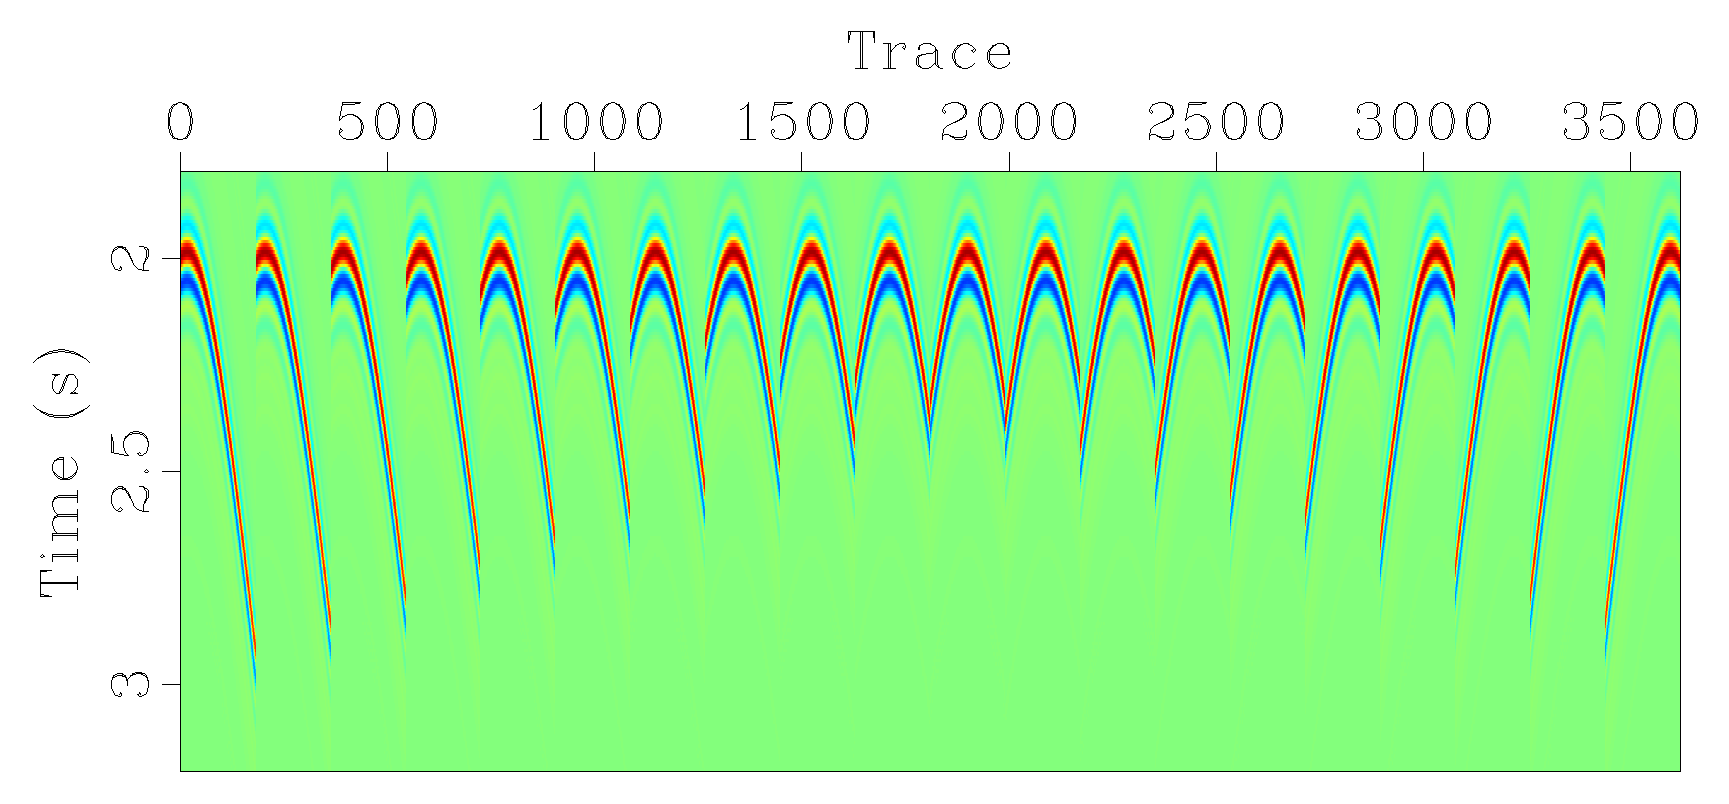
\includegraphics[width=\textwidth]{project/Fig/chwd20}
\caption{Data from the homogeneous model $m_0$ acquired using 20 sources located along a vertical line at $x=3000$ m and 181 receivers at $x=5000$ m.}
\label{fig:chwd20}
\end{center}
\end{figure}

%\plot{chwd20}{width=\textwidth}{Data for homogeneous model $m_0$: 20
%sources at $x=3000$ m, 201 receivers at $x=5000$ m.}

We apply a version of weighted steepest descent optimization to the
minimization of both $J_{\rm FWI}$ and $\tilde{J}_{\alpha,\sigma}$.
The inverse weight operator ($W^{-1}$
in formula \ref{eqn:fwiwgrad}) is a
10-point moving average in both spatial directions, repeated once,
except in the fourth example as discussed below. Recall that the weight operator itself is not required. The weighted
gradient is computed via formula \ref{eqn:fwigrad}. The adjoint
derivative $DF[m]^T$ is computed via the {\em adjoint state method}
\cite[]{Chavent:74,GauTarVir:86}, with time reversal of the acoustic fields
implemented via optimal checkpointing
\cite[]{Griewank:92,Griewank:book,Symes:06a-pub}. The negative of the weighted
gradient ($g_W$, formula \ref{eqn:fwiwgrad}) is the search direction,
and the optimal step in this direction is approximated by a simple
backtracking line search algorithm \cite[]{NocedalWright}. The
iteration is terminate either when the gradient norm has fallen below
1\% of its initial value, or when a maximum number of iterations
(usually 12) is reached.

The MSWI objective $\tilde{J}_{\alpha,\sigma}$ requires choices of the
parameters $\alpha$ and $\sigma$, and solution of the normal equation
\ref{eqn:normal}. This system is far larger than is convenient to solve
by any variant of Gaussian Elimination, even for our small 2D
examples, so iterative methods are 
necessary. We choose the Conjugate Gradient (CG.) method
\cite[]{Dan:67,Steihaug:83,NocedalWright}, and stop the
iteration by monitoring the reduction in length of the normal residual
(the gradient of $J_{\alpha,\sigma}[m,u;d]$ with respect to $u$). The
reduction threshhold $\rho$ is thus another necessary input
parameter. For all calculations in this paper, we use
we choose $\rho = 0.01$ (note that unlike $\alpha$ and $\sigma$,
$\rho$ is dimensionless).

Choice of regularization weights like $\alpha$ and $\sigma$ is a
widely studied topic; we mention some methods for this task in the
discussion section. For the set of examples presented here, we take a
simpler approach. Since the purpose of $\sigma>0$ is to avoid singularity
in the system \ref{eqn:normal} even for $\alpha=0$, we choose it a bit
bigger than floating point tolerance for single precision:
$\sigma = 10^{-5}$. We choose $\alpha$ by computing the solution
$u_{\alpha,\sigma}[m_0;d]$ for the data $d$ used in the first example
below, and several powers of 10 for $\alpha$. The largest such
$\alpha$ that yields an RMS predicted data error
($\|S[m_0]u_{\alpha,\sigma}[m_0;d] - d\|$) less than $0.05 \|d\|$ is
$\alpha = 10^{-4}$. We take this relation as representative, and use
this value for all MSWI computations.

\subsection{Recovering a circular lens}

The target bulk modulus field ($\kappa$) for the first example 
is depicted in Figure \ref{fig:m}. It contains an acoustic ``lens''
positioned in the center between 1000 m and 3000 m depth
(``$z$''). The background level outside the lens is 4 GPa; at the
center it is 2.4 GPa. The
buoyancy ($\beta$)is spatially homogeneous at 1 cm$^3/g$, so the background
wave speed is 2000 m/s.

\plot{m}{width=\textwidth}{Lens model.}

Simulated data from this configuration appears as Figure
\ref{fig:cwd20}.

\plot{cwd20}{width=\textwidth}{Data for circular lens model (\ref{fig:m}): 20
  sources at $x=3000$ m, 201 receivers at $x=5000$ m.}

The value of $J_{\rm FWI}[m_0,d] \approx 4.6$, and the rate of
increase in the weighted gradient direction at $m_0$ is 4.2 $\times
10^{-6 }$. Note that the rate of increase is the same as the weighted
gradient norm. After 12 steepest descent steps, the objective value has
decreased to 2.6, and the
weighted gradient norm by more than an order of magnitude, to $\approx 2.5 \times 10^{-7}$. The
final model appears in Figure \ref{fig:cwlens20mestfwi0}, and the
corresponding data in Figure \ref{fig:cwlens20resimmestfwi0}.

%\multiplot{2}{mestfwi0,resimfwi0}{width=0.45\textwidth}{a: Bulk
%  modulus produced by 10 steepest descent steps to minimize the FWI
%  objective $J_{\rm FWI}[\cdot;d]$ with data $d$ depicted in Figure
%  \ref{fig:sim11}, starting with homogeneous model. b: Data simulated
%  from FWI inversion result.}

\plot{cwlens20mestfwi0}{width=\textwidth}{a: Bulk modulus produced by 10
  steepest descent steps to minimize the FWI objective \ref{eqn:fwi},
  using the data shown in \ref{fig:cwd20}.}

\multiplot{2}{cwlens20resimmestfwi0,cwlens20residmestfwi0}{width=0.45\textwidth}{a: Data
  corresponding to FWI inversion result shown in Figure
  \ref{fig:cwlens20mestfwi0}. b: Residual or data error - difference between
  data shown in Figure \ref{fig:cwlens20resimmestfwi0} and target data
  \ref{fig:cwd20}. Note the failure to match arrival times of the later signal in the
  central part of the display.}

While the reduction in the (weighted) gradient norm indicates progress
towards a stationary point, it is not possible to claim that the final
estimate is in the vicinity of a local minimizer. The fit to data
obtained is not at all satisfactory. More discussion of this result
will be found below.

This example is the one on which we based the choice $\alpha =
10^{-4}$. We did this by minimizing $J_{\alpha,\sigma}[m_0, u; d]$
over $u$ to identify a filter that outputs a good fit to the data
\ref{fig:cwd20} from the input \ref{fig:chwd20} (simulated from
$m_0$), and choosing $\alpha$ just small enough to obtain an RMS error
under 5\%.  The resulting adaptive filter $u_{\alpha,\sigma}[m_0;d]$
is shown in Figure \ref{fig:cwlens20uest0}. This filter exhibits a lot
of energy at non-zero times, as is necessary to move the events in
\ref{fig:chwd20} near those in \ref{fig:cwd20}. Thus the penalty term
is rather large. We will use the apparent dispersion of energy away
from $t=0$ in these adaptive filters to judge the quality of
inversions.

\plot{cwlens20uest0}{width=\textwidth}{Adaptive filter to match
  initial model data (Figure \ref{fig:chwd20}) to circular lens
  data (Figure \ref{fig:cwd20}). Note considerable energy dispersion
  away from $t=0$.}

We applied the same steepest descent algorithm to the MSWI objective
$J_{\alpha,\sigma}$. The initial bulk modulus field is once again
homogeneous at 4 GPa. The initial value of the reduced MSWI objective
is $\approx 1.49 \times 10^{-2}$, and the length of the (weighted)
gradient is $\approx 4.7 \times 10^{-10}$. After 12 iterations, the value has
decreased to $\approx 3.25 \times 10^{-3}$, or roughly a factor of 4.5.
reduction. The gradient length is
$\approx 5.6 \times 10^{-12}$, a reduction of almost two orders of
magnitude. The resulting bulk modulus is shown in Figure
\ref{fig:cwlens20mestmswi}.

\plot{cwlens20mestmswi}{width=\textwidth}{a: Bulk modulus produced by 12
  steepest descent steps to minimize the reduced MSWI objective \ref{eqn:redfiltpen},
  using the data shown in \ref{fig:cwd20}.}

The final adaptive filter is shown in Figure
\ref{fig:cwlens20uestmswi}. Note that energy in the filter has
migrated towards $t=0$, compared to the adaptive filter produced from
the homogenous bulk modulus \ref{fig:cwlens20uest0}, and the bulk of
it is within an apparent half-wavelength of $t=0$. This suggests that
the MSWI result may be an adequate initial estimate for a successful
FWI.

\plot{cwlens20uestmswi}{width=\textwidth}{Adaptive filter to match
  data for MSWI model (Figure \ref{fig:cwlens20resimmestmswi}) to circular lens
  data (Figure \ref{fig:cwd20}). Note considerable less energy dispersion
  away from $t=0$ than is evident in Figure \ref{fig:cwlens20uest0}.}

Another way to look at the improved data kinematics of the MSWI result
is via the simulate data from the model shown in
\ref{fig:cwlens20mestmswi}. Figures \ref{fig:cwlens20resimmestmswi},
\ref{fig:cwlens20residmestmswi} suggest that the
data predicted from the MSWI result is in many places within a
half-wavelength travel time shift of the data in Figure \ref{fig:cwd20}.
A half-wavelength is the conventional threshhold for FWI initial fit
error: below that it works, above that it doesn't.

\multiplot{2}{cwlens20resimmestmswi,cwlens20residmestmswi}{width=0.45\textwidth}{a:
  Data corresponding to MSWI result shown in Figure
  \ref{fig:cwlens20mestmswi}. b: Residual or data error - difference between
  data shown in Figure \ref{fig:cwlens20resimmestmswi} and target data
  \ref{fig:cwd20}. Note that the later signal in the central portion is
  still shifted, but by much less than in Figure \ref{fig:cwlens20residmestfwi0}.}

We applied 11 iterations of steepest descent to the FWI objective,
with initial estimate of $m$ equal to the final estimate from the MSWI
inversion just described (Figure \ref{fig:cwlens20mestmswi}). The initial FWI
objective value was $\approx 2.9$, and the weighted gradient norm was
$\approx 2.0 \times 10^{-4}$.  After 11 steps of steepest descent,
the prescribed reduction ($10^{-2}$) of the weighted gradient norm was achieved,
and the objective value had decreased to $\approx 9.1 \times
10^{-2}$. The resulting bulk modulus field is depicted in Figure
\ref{fig:cwlens20mestmswifwi}. The predicted data at this model, and the residual
data, are shown in Figures \ref{fig:cwlens20resimmestmswifwi} and \ref{fig:cwlens20residmestmswifwi}
respectively.

\plot{cwlens20mestmswifwi}{width=\textwidth}{a: Bulk modulus produced by 11
  steepest descent steps to minimize the FWI objective \ref{eqn:fwi},
  using the data shown in \ref{fig:cwd20}, and starting at the MSWI
  result shown in Figure \ref{fig:cwlens20mestmswi}. Reduction in
  gradient norm of 2 orders of magnitude.}

\multiplot{2}{cwlens20resimmestmswifwi,cwlens20residmestmswifwi}{width=0.45\textwidth}{a: Data
  corresponding to FWI result shown in Figure
  \ref{fig:cwlens20mestmswifwi}. b: Residual or data error - difference between
  data shown in Figure \ref{fig:cwlens20resimmestmswifwi} and target data
  \ref{fig:cwd20}.}

Yet another way to examine the kinematic fit between the target data
and the resimulated data (Figure \ref{fig:cwlens20resimmestmswifwi})
is via the adaptive filter computed with the FWI + MSWI model (Figure
\ref{fig:cwlens20mestmswifwi}).  Figure \ref{fig:cwlens20uest1}
shows how precisely the kinematics of the resimulation match those of
the target data.

\plot{cwlens20uest1}{width=\textwidth}{Adaptive filter to match
  data for FWI + MSWI model (Figure \ref{fig:cwlens20resimmestmswi}) to circular lens
  data (Figure \ref{fig:cwd20}). Dispersion away from 
  away from $t=0$ has almost disappeared, showing that the resimulated
  data is nearly a perfect kinematic match with the target data.}

The FWI iteration starting at the MSWI result has effectively achieved
the global minimum of the FWI objective function: the data match is
very close. The combination of MSWI followed by FWI has fit the data
starting from the homogeneous initial model, a result that was not obtained
by FWI alone with the algorithmic choices made here.

\subsection{Oblate lens: single vs. multiple arrivals}

Our next two examples use another lens model, somewhat deeper (with a
minimum bulk modulus of 2 GPa in the center), therefore more
refractive, and extended in the
horizontal direction. See Figure \ref{fig:dcwm}. As is the case with
the circular lens, this oblate lens is smooth to adequate numerical
approximation.

\plot{dcwm}{width=\textwidth}{Oblate lens model.}

The first example using this model has exactly the same acquisition
geometry as was used in the circular lens example: 20 sources at x =
3000 m, 201 receivers at x = 5000 m, spaced as described in the
previous section. The data is shown in Figure \ref{fig:dcowd20}. 

\plot{dcowd20}{width=\textwidth}{Data using model shown in Figure
  \ref{fig:dcwm}, same source-receiver geometry as for circular lens
  data (Figure \ref{fig:cwd20}).}

The stronger refraction produced by this model produces a visible triplication
the center of the source-receiver line, and in fact in all parts of
the data, although the smearing effect of finite bandwidth obscures this
detail in many placed. So most of the data can be (just!) regarded as exhibiting a single
arrival on an identifiable wavefront.

In this and subsequent examples, FWI initiated from the homogeneous
model fails in the same way as shown in the  previous section. So
there is no point in showing the results, and we don't.

Application of steepest descent to the MSWI objective (with the same
parameters as in the previoius example) results in the model depicted
in Figure \ref{fig:mnqcaustic20mestmswi}, and reduces the objective to
roughly 20\% of its initial value, and the gradient norm to 7.5\%. Data
simulated with this model is shown in Figure
\ref{fig:mnqcaustic20resimmestmswi}, and the residual in Figure
\ref{fig:mnqcaustic20residmestmswi}.

\plot{mnqcaustic20mestmswi}{width=\textwidth}{Result of 8 MSWI
  iterations applied to the data in Figure \ref{fig:dcowd20}, beginning
  at the homogeneous model.}

\multiplot{2}{mnqcaustic20resimmestmswi,mnqcaustic20residmestmswi}{width=0.45\textwidth}{a: Data
  corresponding to MSWI result shown in Figure
  \ref{fig:mnqcaustic20mestmswi}. b: Residual or data error - difference between
  data shown in Figure \ref{fig:mnqcaustic20resimmestmswi} and target data
  \ref{fig:dcowd20}.}

The change in adaptive filters between the homogenous initial model
and the MSWI inversion is shown in Figures
\ref{fig:mnqcaustic20uest0} and \ref{fig:mnqcaustic20uestmswi}. The
reduction in energy dispersion is evident.

\multiplot{2}{mnqcaustic20uest0,mnqcaustic20uestmswi}{width=0.45\textwidth}{a:
  adaptive filter estimate for homogeneous initial model, data of
  Figure \ref{fig:dcowd20}; b: adaptive filter estimate for MSWI
  inversion shown in Figure \ref{fig:mnqcaustic20mestmswi}.}

These results render the MSWI inversion result a plausible initial
estimate for FWI. Twelve FWI iterations applied to the data in Figure \ref{fig:dcowd20}, starting at the model of
Figure \ref{fig:mnqcaustic20mestmswi}, result in the
model shown in Figure \ref{fig:mnqcaustic20mestmswifwi}, at which the
FWI objective has decreased to 4\% of its initial value. That is, the
RMS error between data and predicted data has been reduced to
approximately 20\% of its initial value; the gradient
decreases by a slightly larger factor. The reduction obtained is evident in the plots of simulated data and
residual (Figures \ref{fig:mnqcaustic20resimmestmswifwi} and
\ref{fig:mnqcaustic20residmestmswifwi}). Residual energy is
concentrated in later arrivals in the
central zone, suggesting that the model shown in Figure
\ref{fig:mnqcaustic20mestmswifwi} may lie in the basin of global minimization. Finally, energy dispresion
from $t=0$ has nearly disappeared from the adaptive filter computed
from this FWI +MSWI result, again except for some traces in the
central zone (Figure \ref{fig:mnqcaustic20uest1}).

\plot{mnqcaustic20mestmswifwi}{width=\textwidth}{a: Bulk modulus produced by 12
  steepest descent steps to minimize the FWI objective \ref{eqn:fwi},
  using the data shown in \ref{fig:dcowd20}, and starting at the MSWI
  result shown in Figure \ref{fig:mnqcaustic20mestmswi}.}

\multiplot{2}{mnqcaustic20resimmestmswifwi,mnqcaustic20residmestmswifwi}{width=0.45\textwidth}{a: Data
  corresponding to FWI + MSWI result shown in Figure
  \ref{fig:mnqcaustic20mestmswifwi}. b: Residual or data error - difference between
  data shown in Figure \ref{fig:mnqcaustic20resimmestmswifwi} and target data
  \ref{fig:dcowd20}.}

\plot{mnqcaustic20uest1}{width=\textwidth}{Adaptive filter to match
  data for FWI + MSWI model (Figure \ref{fig:mnqcaustic20resimmestmswi}) to oblate lens
  data (Figure \ref{fig:dcowd20}). Dispersion away from 
  away from $t=0$ has almost disappeared, showing that the resimulated
  data is nearly a perfect kinematic match with the target data.}

The second example based on the target model in Figure \ref{fig:dcwm}
differs from the first {\em only} in that the sources and receivers
have been moved further away from each other: the sources lie on the
line $x=2000$, the receivers on $x=6000$. That is, the source-receiver
offset has been doubled. Otherwise, all aspects of data generation are
the same, and produce the data shown in Figure \ref{fig:dcwd20}.

\plot{dcwd20}{width=\textwidth}{Data generated using the same inputs
  as in Figure \ref{fig:dcowd20}, but with sources moved to $x=2000$
  and receivers to $x=6000$.}

Notice that the additional offset has allowed distinct energetic later
arrivals to appear in the data.

As before, we compute the adaptive filter required to produce the data
of Figure \ref{fig:dcwd20} from the corresponding homogeneous medium data (Figure
\ref{fig:chwd20}). This filter, displayed in \ref{fig:mcaustic20uest0},
shows that for most traces, two or more major energy peaks appear in the
adaptive filter, forced by the need to match multiple energy peaks in
the target data with the single energy peak in the homogeneous medium
data.

Using the same parameters (tolerance of 0.01 for the normal residual
in the CG iteration, same smoothing operator as inverse weight
defining norm in model space) 12 steps of steepest descent applied to
the MSWI objective produces the model
estimate depicted in Figure \ref{fig:mcaustic20mestmswi}. The overall
decrease in bulk modulus is correct, but the minimum bulk modulus attained (2.8 GPa) is considerably larger
than the target's, and moreover is concentrated around the source
line, suggesting that the amount of refraction produced by this model is
considerably less. That guess is verified by resimulating the data
(Figure \ref{fig:mcaustic20resimmestmswi}): the predicted data does not
exhibit triplication. The computed adaptive filter (Figure 
\ref{fig:mcaustic20uestmswi}) appears to attempt a compromise between
earlier and later arrivals. Most importantly, the final gradient norm
is approximately 18\% of the initial, suggesting that the minimizer has
not been approximated as well as was the case in the previous
examples. FWI initiated at the MSWI estimate gives an evidently
cycle-skipped model estimate (Figure \ref{fig:mcaustic20mestmswifwi}),
with unsatisfactory resimulation and residual (Figures
\ref{fig:mcaustic20resimmestmswifwi},
\ref{fig:mcaustic20residmestmswifwi}), and considerable energy spread
ion the estimated adaptive filter (Figure \ref{fig:mcaustic20uest1}.

\plot{mcaustic20uest0}{width=\textwidth}{Adaptive filter required to produce the data
of Figure \ref{fig:dcwd20} from corresponding homogeneous medium data (Figure
\ref{fig:chwd20}).}


\plot{mcaustic20mestmswi}{width=\textwidth}{Result of 12 MSWI
  iterations applied to the data in Figure \ref{fig:dcwd20}, beginning
  at the homogeneous model.}

\multiplot{2}{mcaustic20resimmestmswi,mcaustic20residmestmswi}{width=0.45\textwidth}{a: Data
  corresponding to MSWI result shown in Figure
  \ref{fig:mcaustic20mestmswi}. b: Residual or data error - difference between
  data shown in Figure \ref{fig:mcaustic20resimmestmswi} and target data
  \ref{fig:dcwd20}.}

\plot{mcaustic20uestmswi}{width=\textwidth}{Adaptive filter estimate for MSWI
  inversion shown in Figure \ref{fig:mcaustic20mestmswi}.}

\plot{mcaustic20mestmswifwi}{width=\textwidth}{Bulk modulus produced by 12
  steepest descent steps to minimize the FWI objective \ref{eqn:fwi},
  using the data shown in \ref{fig:dcwd20}, and starting at the MSWI
  result shown in Figure \ref{fig:mcaustic20mestmswi}.}

\multiplot{2}{mcaustic20resimmestmswifwi,mcaustic20residmestmswifwi}{width=0.45\textwidth}{a: Data
  corresponding to FWI + MSWI result shown in Figure
  \ref{fig:mcaustic20mestmswifwi}. b: Residual or data error - difference between
  data shown in Figure \ref{fig:mcaustic20resimmestmswifwi} and target data
  \ref{fig:dcwd20}.}

\plot{mcaustic20uest1}{width=\textwidth}{Adaptive filter to match
  data for FWI + MSWI model (Figure \ref{fig:mcaustic20resimmestmswi}) to oblate lens
  data (Figure \ref{fig:dcwd20}). Considerable energy dispersion away
  from $t=0$ remains, showing that the inverted model does not match
  data kinematics well.}

As noted above, the reduction in MSWI gradient norm achieved in 12 steepest
descent iterations for this example is not as great as was the case in
the two previous exmaples: this appears to be a more difficult
optimization. Accordingly, we perform 12 additional iterations of
steepest descent applied to the MSWI objective, starting withe the
result (Figure \ref{fig:mcaustic20mestmswi}) of the first 12
iterations. The objective decreases by roughly 0.8, the gradient by
0.5. Inspection of the model so obtained (Figure
\ref{fig:mcaustic20mestmswicont}) shows that the minimum bulk modulus
has decreased (2.09 GPa, vs 2.8  GPa at the
end of the first 12 iterations), however the smallest values are even
more concentrated around the source locations, and the resimulated
data with this model is if anything less similar to the data than was
the case at the end of the first 12 iterations (Figures
\ref{fig:mcaustic20resimmestmswicont},
\ref{fig:mcaustic20residmestmswicont}). The adaptive filter is no more
focused at $t=0$ than was the case at the end of the first 12
iterations: it appears to have adjusted the compromise between shifts
to fit early and late arrivals, nothing more (Figure \ref{fig:mcaustic20uestmswicont}). 

\plot{mcaustic20mestmswicont}{width=\textwidth}{Result of 24 MSWI
  iterations applied to the data in Figure \ref{fig:dcwd20}, beginning
  at the homogeneous model.}

\multiplot{2}{mcaustic20resimmestmswicont,mcaustic20residmestmswicont}{width=0.45\textwidth}{a: Data
  corresponding to MSWI result shown in Figure
  \ref{fig:mcaustic20mestmswicont}. b: Residual or data error - difference between
  data shown in Figure \ref{fig:mcaustic20resimmestmswicont} and target data
  \ref{fig:dcwd20}.}

\plot{mcaustic20uestmswicont}{width=\textwidth}{Adaptive filter estimate for MSWI
  inversion shown in Figure \ref{fig:mcaustic20mestmswicont}.}

This result (Figure \ref{fig:mcaustic20mestmswicont}) is actually a
{\em worse} initial estimate for FWI than was the model obtained after
12 steepet descent iterations. We
performed 25 steps of steepest descent applied to the FWI objective
with the model in Figure \ref{fig:mcaustic20mestmswicont} as initial
estimate, resulting in the obviously cycle-skipped model displayed in
Figure \ref{fig:mcaustic20mestmswifwicont}. The residual (Figure
\ref{fig:mcaustic20residmestmswifwicont} and adaptive filter (Figure
\ref{fig:mcaustic20uest2}) have actually deteriorated relative to
those obtained before.

\plot{mcaustic20mestmswifwicont}{width=\textwidth}{Bulk modulus produced by 25
  steepest descent steps to minimize the FWI objective \ref{eqn:fwi},
  using the data shown in \ref{fig:dcwd20}, and starting at the MSWI
  result shown in Figure \ref{fig:mcaustic20mestmswicont}.}

\multiplot{2}{mcaustic20resimmestmswifwicont,mcaustic20residmestmswifwicont}{width=0.45\textwidth}{a: Data
  corresponding to FWI + MSWI result shown in Figure
  \ref{fig:mcaustic20mestmswifwicont}. b: Residual or data error - difference between
  data shown in Figure \ref{fig:mcaustic20resimmestmswifwicont} and target data
  \ref{fig:dcwd20}.}

\plot{mcaustic20uest2}{width=\textwidth}{Adaptive filter to match
  data for FWI + MSWI model (Figure \ref{fig:mcaustic20resimmestmswicont}) to oblate lens
  data (Figure \ref{fig:dcwd20}). Dispersion away from 
  away from $t=0$ has almost disappeared, showing that the resimulated
  data is nearly a perfect kinematic match with the target data.}

The meaning of this result will be discussed further below. For now
merely note that the first example based on the oblate lens model in
Figure \ref{fig:dcwm} appeared to require more computational effort
than the cirular lens example to achieve a successful inversion,
whereas the second was an inversion failure even with considerably
more effort.

\subsection{Recovering a Camembert: effect of non-smoothness}

\plot{cambulk}{width=\textwidth}{A model resembling the ``camembert''
  of \cite{GauTarVir:86}. Diameter of circular inclusion = 2500 m,
  approximately 8 wavelengths at median frequency. Interior value 20\%
above exterior (4.8 GPa vs 4.0 GPa).}

\plot{camcwd20}{width=\textwidth}{Data generated using ``camembert''
  model (Figure \ref{fig:cambulk}), same source-receiver geometry as
  in Figure \ref{fig:dcwd20}: 20 sources located at $x=2000$ m, spaced
  150 m apart, starting at $z=500$ m; 201 receivers located at $x=6000$ m,
  spaced 20 m apart, starting at $z=200$ m.}

\plot{cam20uest0}{width=\textwidth}{Adaptive filter required to produce the data
of Figure \ref{fig:camcwd20} from corresponding homogeneous medium data (Figure
\ref{fig:chwd20}).}

\plot{cam20mestmswi}{width=\textwidth}{Result of 12 MSWI
  iterations applied to the data in Figure \ref{fig:camcwd20}, beginning
  at the homogeneous model.}

\multiplot{2}{cam20resimmestmswi,cam20residmestmswi}{width=0.45\textwidth}
{a: Data  corresponding to MSWI result shown in Figure
  \ref{fig:cam20mestmswi}. b: Residual or data error - difference between
  data shown in Figure \ref{fig:cam20resimmestmswi} and target data
  \ref{fig:camcwd20}.}

\plot{cam20uestmswi}{width=\textwidth}{Adaptive filter estimate for MSWI
  inversion shown in Figure \ref{fig:cam20mestmswi}.}

\plot{cam20mestmswifwi}{width=\textwidth}{Bulk modulus produced by 12
  steepest descent steps to minimize the FWI objective \ref{eqn:fwi},
  using the data shown in \ref{fig:camcwd20}, and starting at the MSWI
  result shown in Figure \ref{fig:cam20mestmswi}.}

\multiplot{2}{cam20resimmestmswifwi,cam20residmestmswifwi}{width=0.45\textwidth}{a: Data
  corresponding to FWI + MSWI result shown in Figure
  \ref{fig:cam20mestmswifwi}. b: Residual or data error - difference between
  data shown in Figure \ref{fig:cam20resimmestmswifwi} and target data
  \ref{fig:camcwd20}.}

\plot{cam20uest1}{width=\textwidth}{Adaptive filter to match
  data for FWI + MSWI model (Figure \ref{fig:cam20resimmestmswi}) to ``camembert'' 
  data (Figure \ref{fig:camcwd20}).}

\plot{cam20mestmswifwifine}{width=\textwidth}{``Hi-res'' bulk modulus produced by
  25 additional steepest descent steps, with inverse weight operator =
  2 point moving average in both directions, repeated once, and
  initial bulk modulus = output of first FWI + MSWI cycle (Figure
  \ref{fig:cam20mestmswifwi}). Note that top and bottom edges of disk
  shown in Figure \ref{fig:cambulk} are clearly visible.}

\multiplot{2}{cam20resimmestmswifwifine,cam20residmestmswifwifine}{width=0.45\textwidth}{a: Data
  corresponding to hi-res FWI + MSWI result shown in Figure
  \ref{fig:cam20mestmswifwifine}. b: Residual or data error - difference between
  data shown in Figure \ref{fig:cam20resimmestmswifwifine} and target data
  \ref{fig:camcwd20}.}

\plot{cam20uest2}{width=\textwidth}{Adaptive filter to match
  data for hi-res FWI + MSWI model (Figure \ref{fig:cam20resimmestmswi}) to ``camembert'' 
  data (Figure \ref{fig:camcwd20}).}


\subsection{Noise}



\section{Discussion}
Several matters deserve attention: character of the FWI result; choice of parameters in the
definition of the MSWI objective; and application to inverse problems
defined by other types of wave physics.

\subsection{FWI failure - local mins?}
The result shown in Figure \ref{fig:cwlens20mestfwi0} is certainly
unsatisfactory, as is evident from the residual plot (Figure
\ref{fig:cwlens20residmestfwi0}). However one cannot conclude {\em
  from this result alone} that further
iterations of steepest descent, or of a more sophisticated local
optimization algorithm, starting at the same homogeneous initial
estimate, would not eventually meander to a global
minimizer, fitting the data - most importantly, the arrival times -
with the same sort of accuracy that FWI achieves when started at the
MSWI result (Figure \ref{fig:cwlens20mestmswi}). Actually, further iterations don't help
in this instance - at least, not O(10) or O(100) additional
iterations (we tried!). On the other hand, if O($10^6$)
additional iterations {\em would} yield a good invertion, it doesn't matter: such vast amount of computational
work is simply not practical. Nor is it sensible, since alternatives
exist (FWI + MSWI) that accomplish the inversion goal with far less
work.

So: we don't know whether Figure \ref{fig:cwlens20mestfwi0} represents an
approximation to a non-global local minimizer, or not - but it doesn't matter.

\subsection{Parameters}
The roles of parameters $\sigma$ and $\alpha$ are quite
different. Regularization, that is, avoidance of singularity in the
normal equation \ref{eqn:normal}, is the purpose of setting $\sigma >
0$. As formulated here, $\sigma$ is a dimensional parameter. It is
simple to make it dimensionless, and that should be done, so that a
``small'' choice is meaningful.

The penalty parameter $\alpha$ however plays a very different role. In
principle, $\alpha \rightarrow \infty$ should force the adaptive
filter to become ``physical'', which in this case means the identity
operator, i.e. with kernel $\delta(t)$ regardless of source and
receiver, so that the penalty problem becomes identical to FWI.

There are a variety of rules for setting penalty parameters like
$\alpha$, of varying degrees of rigor. The discrepancy concept is one
of these: it is simple to implement, auto-starting for problems like
MSWI, and steers the penalty problem towards its limit. No magic
however: this approach requires the assertion of data error. $\alpha$
is adjusted so that the data error term in \ref{eqn:redfiltpen} or
similar function is close to the posited size. Doing so is quite
simple - see \cite{Fu:Geo17b,SymesMinkoffChen:IP22}. It might be objected that
then one opaque parameter ($\alpha$) has been exchanged for another
unknown one (data error), however it is even possible to turn this
construction around to estimate data error
\cite[]{ChenSymesMinkoff:IMAGE22}. In any case, data error has an
obvious meaning, whether it is a known quantity or not, whereas
$\alpha$ is merely a Lagrange multiplier.

\subsection{Other Physics, Other Data}
Acoustics is seldom exactly the right choice of physics for mechanical
vibration modeling; in many settings, some variant of elastodynamics,
perhaps coupled with acoustics in some regions, is the right
choice. Elastic waves travel at several speeds, intrinsically
providing multiple wavefronts. Extension of MSWI and similar
approahces to elastodynamic inverse problems, either by data mode
separation or some more intrinsic construction, would appear to be a
very important next step, as would application to electromagnetic imaging.

Sensors (and energy sources) are seldom punctual and/or
isotropic. Actual source encountered in lab and field can exhibit
non-trivial radiation patterns or even physical extent non-negligible
on the wavelength scale. Inclusion of more realistic source modeling
also seems a very important next step, even for those problems
admitting a successful approach via source-receiver extension.

As has been emphasized several times, wavefront complexity can prevent
successful application of inversion methods based on source-receiver
extension. A variety of other source extension approaches have been
explored, some with positive numerical results
\cite[]{HuangNammourSymesDollizal:SEG19}. For many of these
approaches, the missing piece is a theoretical justification like that
summarized in equation \ref{eqn:tomo} for MSWI.

Finally, the assumption of smooth material parameter variation is
unlikely to be justified in actual physical media. Sedimentary rocks,
human tissue, manufactured objects all exhibit juxtaposition of
structure at all scales, from long scales modeled by smooth variation,
to sub-wavelength oscillations. Most likely, settings in which
ballistic transmitted waves dominate data energetics will permit more
or less unmodified application of techniques like MSWI, at least to
gain a low-resolution image of wave velocity, bulk modulus,.... However
theoretical results in this direction are absent, as are results on
the related question of applicability of algorithms like MSWI to
predominantly reflected wave data.



\bibliographystyle{seg}
\bibliography{../../bib/masterref}
